\documentclass[12pt]{beamer}

\usepackage[english]{babel}
\usepackage[utf8]{inputenc}
\usepackage[T1]{fontenc}
\usepackage{lmodern}
\usepackage[export]{adjustbox}

\usetheme{Berlin}
\usecolortheme{spruce}
\useoutertheme{infolines}

\title{how do we know how far things are}
\author{Ethan Snyder}
\date{\today}

\begin{document}
%\setbeamertemplate{headline}{}

\begin{frame}
    \titlepage
\end{frame}

\section{Introduction}

    \begin{frame}
        \centering
        \large how do we know how far things are?\\
        \vspace{2em}
        \normalsize this will be our leading question\\
        \vspace{2em}
        enjoy :)
    \end{frame}
    \begin{frame}
        \centering
        parallax, mostly
    \end{frame}
    \subsection{Parallax --- Moving \& Stationary}
        \begin{frame}{parallax} \centering
            this may be what you're picturing :)
            \begin{figure}
                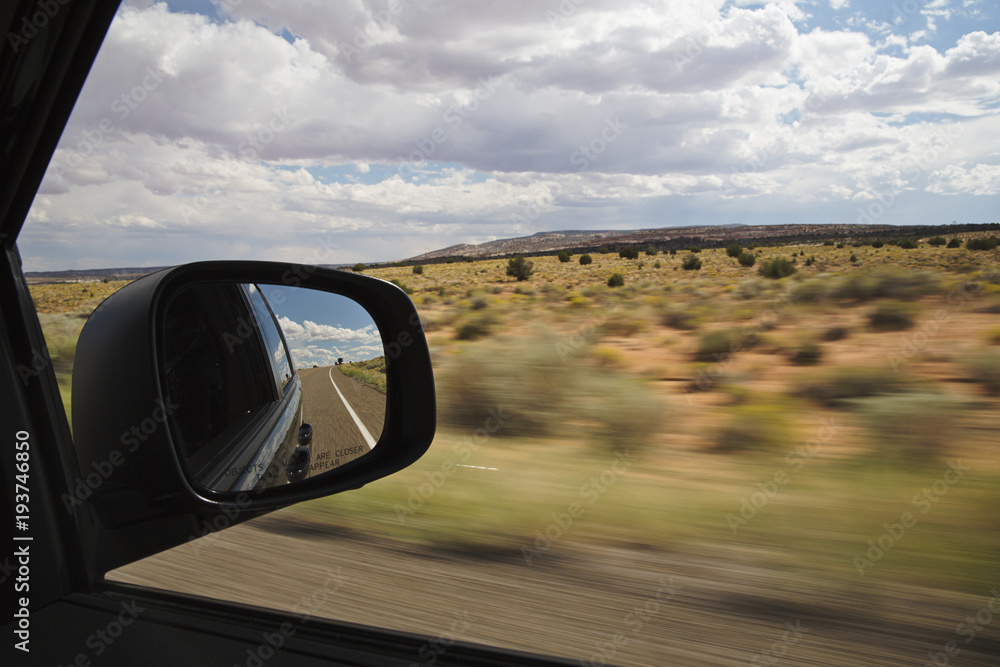
\includegraphics[scale=0.8, fbox, bb=0 0 240 160]{parallaxcar.jpeg}
                \caption{Parallax as seen looking out a moving car's window$^0$.}
            \end{figure}
            \footnotetext{\tiny Image: https://stock.adobe.com/images/view-out-the-car-window-as-the-scenery-blurs-by/193746850}
        \end{frame}
        \begin{frame}{parallax} \centering
            two types of parallax
            \pause
            \begin{columns}
                \begin{column}{0.5\linewidth}
                    \begin{block}{moving parallax}
                        \begin{itemize}
                            \item<3-> involves movement
                            \item<4-> things close to observer appear to move more, things farther appear to move less
                        \end{itemize}
                    \end{block}
                \end{column}
                \begin{column}{0.5\linewidth}
                    \begin{block}{stationary parallax}
                        \begin{itemize}
                            \item<3-> does not
                            \item<4-> the change in an objects appearance from two different locations (at once or at different times)
                        \end{itemize}
                    \end{block}
                \end{column}
            \end{columns}
            \pause[5] \vspace{1em}
            (these are actually the same, kinda. motion is just being in two places at different times :) )
        \end{frame}
        \begin{frame}{moving parallax} \centering
            moving parallax car picture again here look
            \begin{figure}
                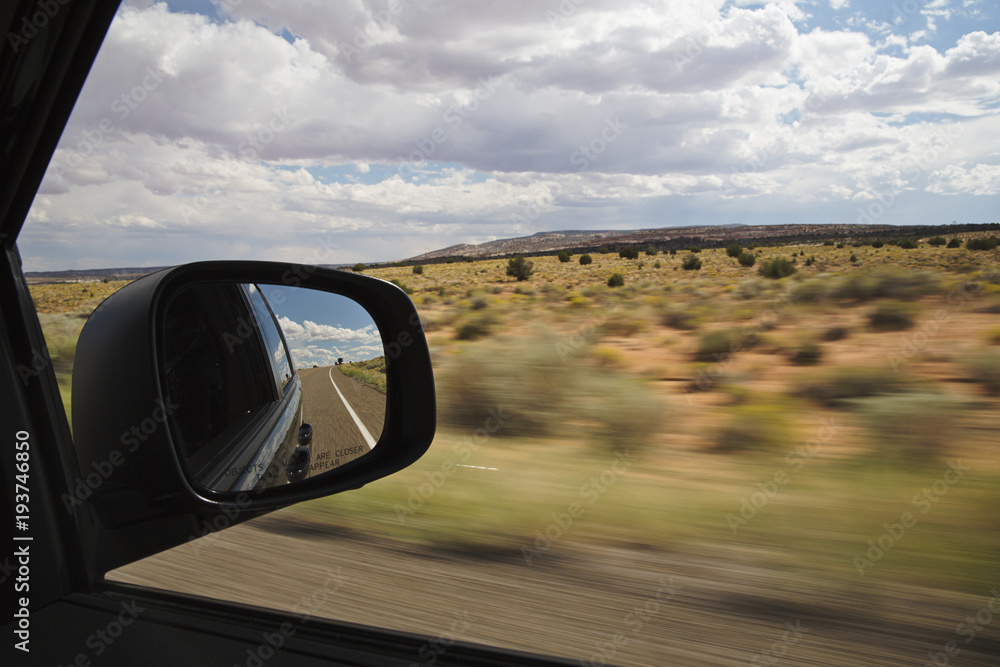
\includegraphics[scale=0.8, fbox, bb=0 0 240 160]{parallaxcar.jpeg}
                \caption{Parallax as seen looking out a moving car's window again$^0$.}
            \end{figure}
            \footnotetext{\tiny Image: https://stock.adobe.com/images/view-out-the-car-window-as-the-scenery-blurs-by/193746850}
        \end{frame}
        \begin{frame}{stationary parallax} \centering
            like human eyes, for example\\
            this is how depth perception works
            \begin{figure}
                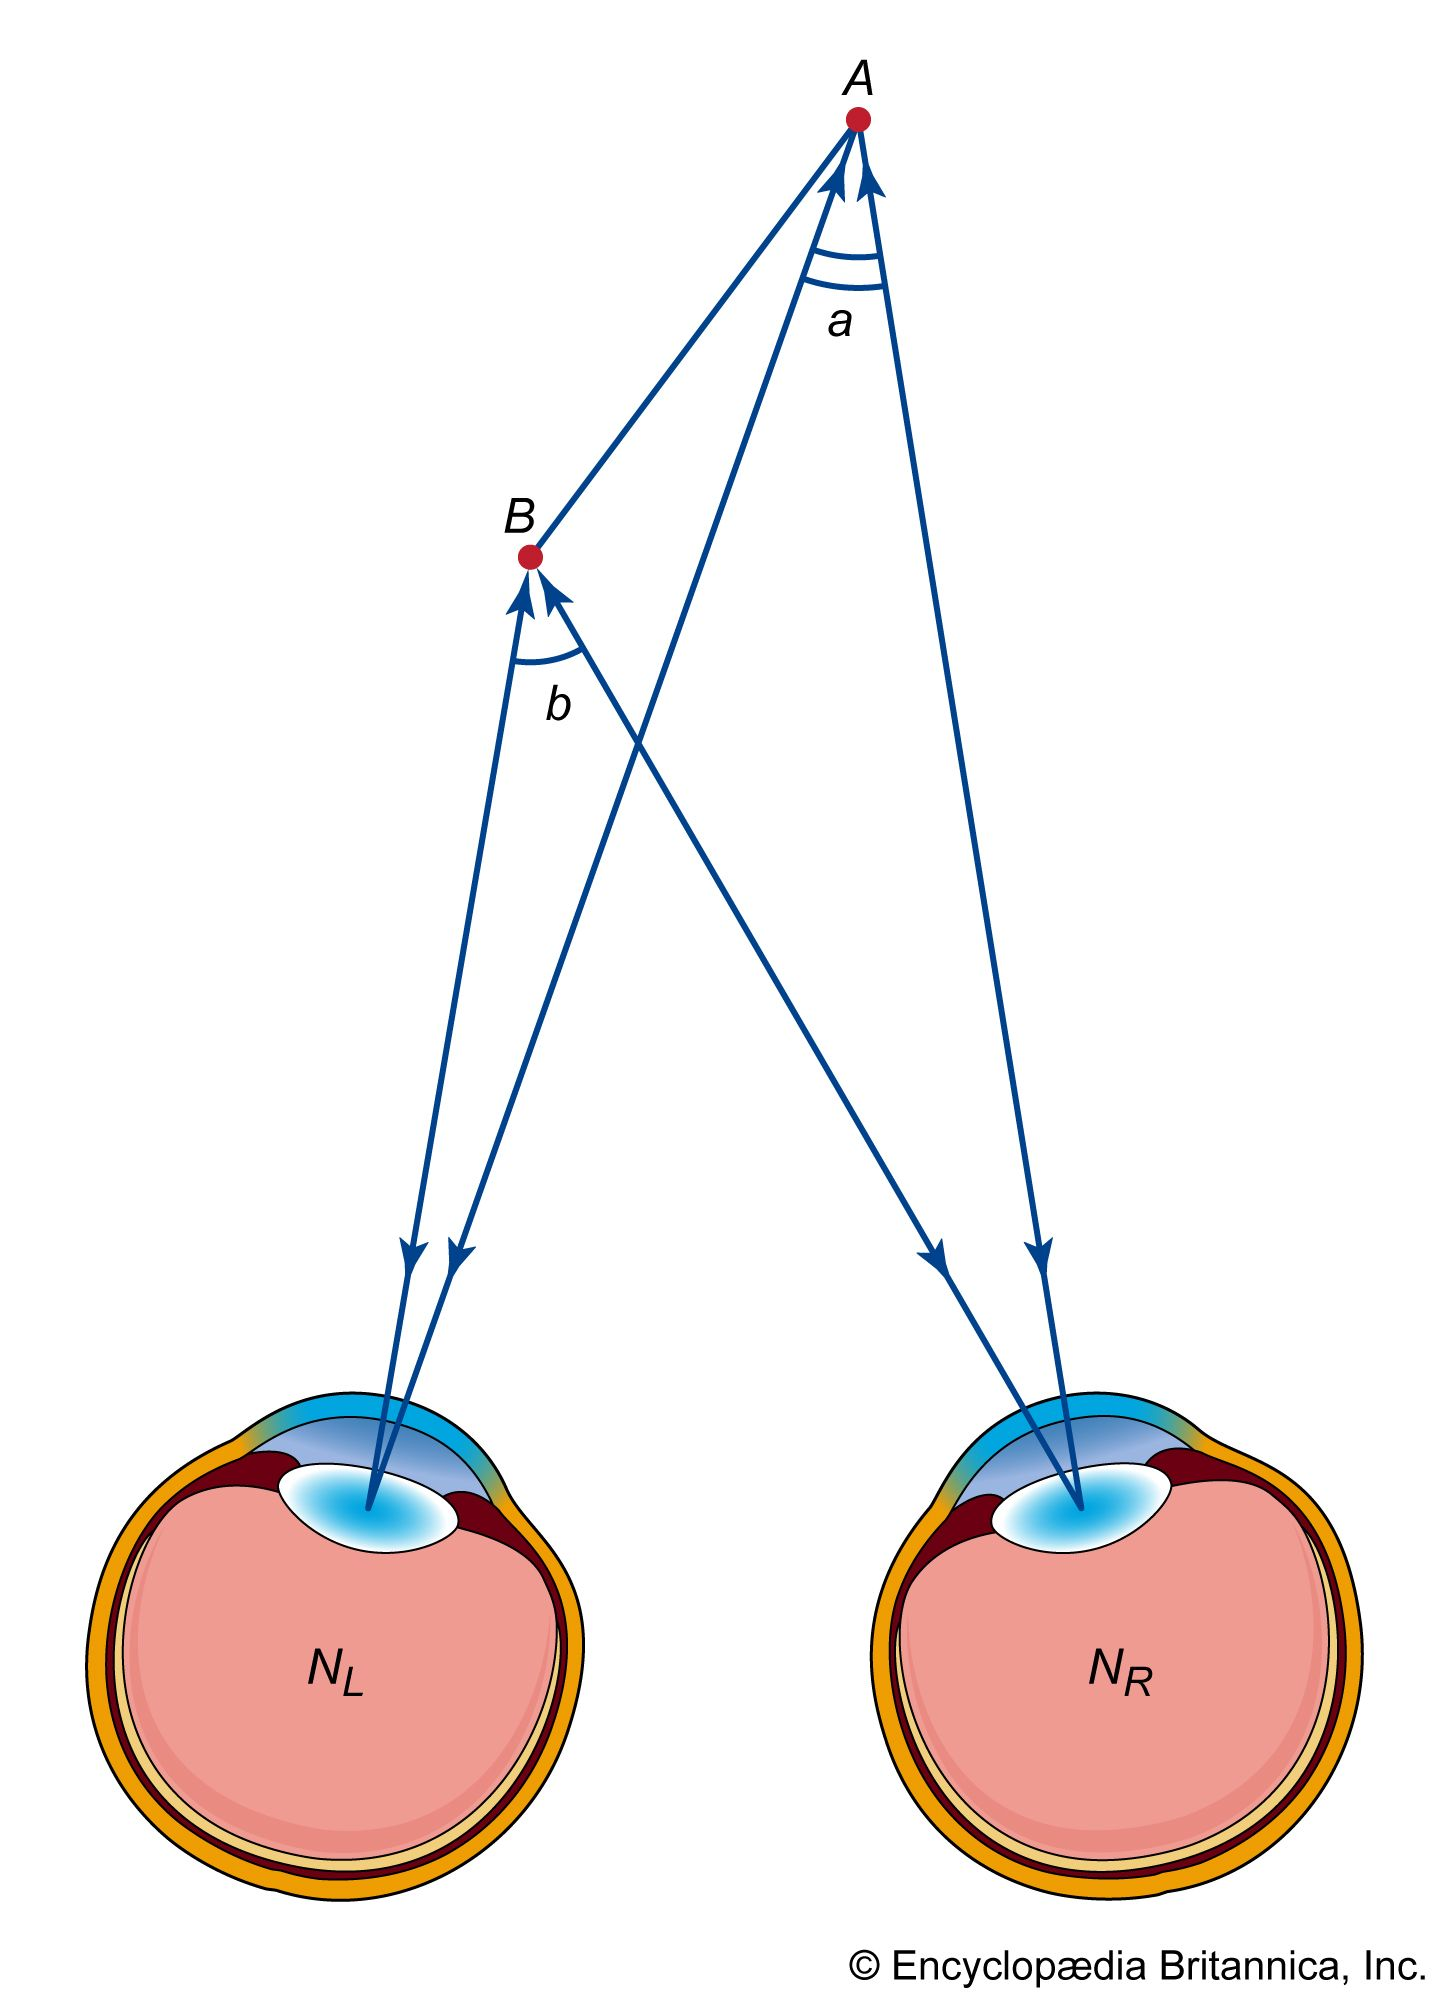
\includegraphics[scale=0.06, bb=0 0 1400 2000, fbox]{parallaxeyes.jpg}
                \caption{Eyes doing parallax$^0$.}
            \end{figure}
            \footnotetext{\tiny Image: https://cdn.britannica.com/85/4085-050-5575ACA3/parallax-points-NL-eyes-NR-left.jpg}
        \end{frame}
        \begin{frame}{summary} \centering
            we know how far things are away from us\\because we have EYES dipshit
        \end{frame}
        \begin{frame} \centering
            ok but what about numbers\\
            \vspace{2em}
            like what if we want to MEASURE a distance
        \end{frame}
        \begin{frame}
            \tableofcontents
        \end{frame}
\section{Measuring Shortish Distances}
    \subsection{Apparent Size, Units, Measuring Devices}
        \begin{frame}{Apparent Size}{What if you \textit{know the size of a distant object?}} \centering
            Easiest solution for measuring a distance.
            \begin{figure}
                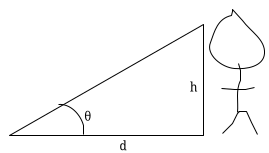
\includegraphics[scale=0.6, bb=0 0 280 160]{angletriangle.png}
            \end{figure}
            \pause
            \[\sin{\theta}=\frac{h}{d} \implies d=\frac{h}{\sin{\theta}}\]
            \pause
            (you just need to know the size of the distant object and be able to measure the \textit{angular extent} $\theta$)
        \end{frame}
        \begin{frame}{dawg wt f}{what if I don't have a protractor or konw the size of the thing?}
            \begin{figure}
                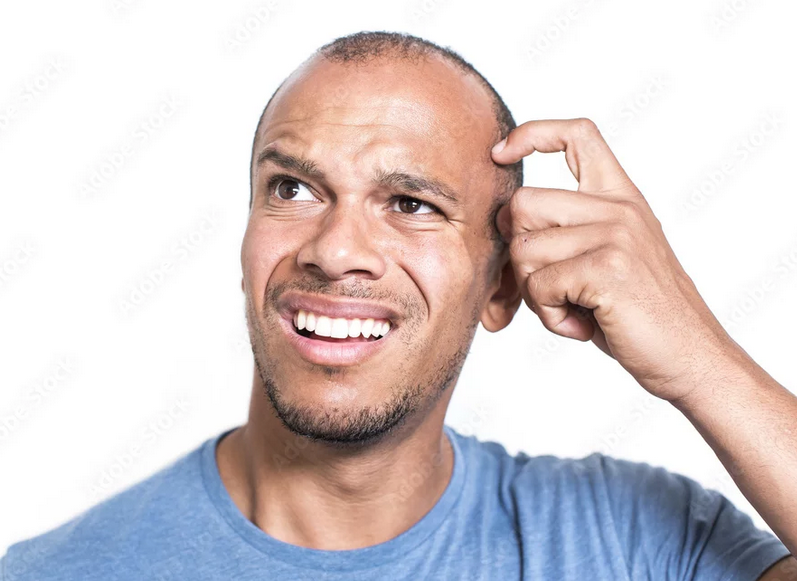
\includegraphics[scale=0.2, bb=0 0 800 600]{confused.png}
                \caption{Man scratching his head, confused about how to measure a distance without prior knowledge of a distant object's size or the ability to measure angular extent$^0$.}
            \end{figure}
            \footnotetext{\tiny Image: https://stock.adobe.com/images/portrait-of-a-mixed-race-man-scratching-his-head-in-confusion/68695988}
        \end{frame}
    \subsection{Units}
        \begin{frame}
            \begin{figure}
                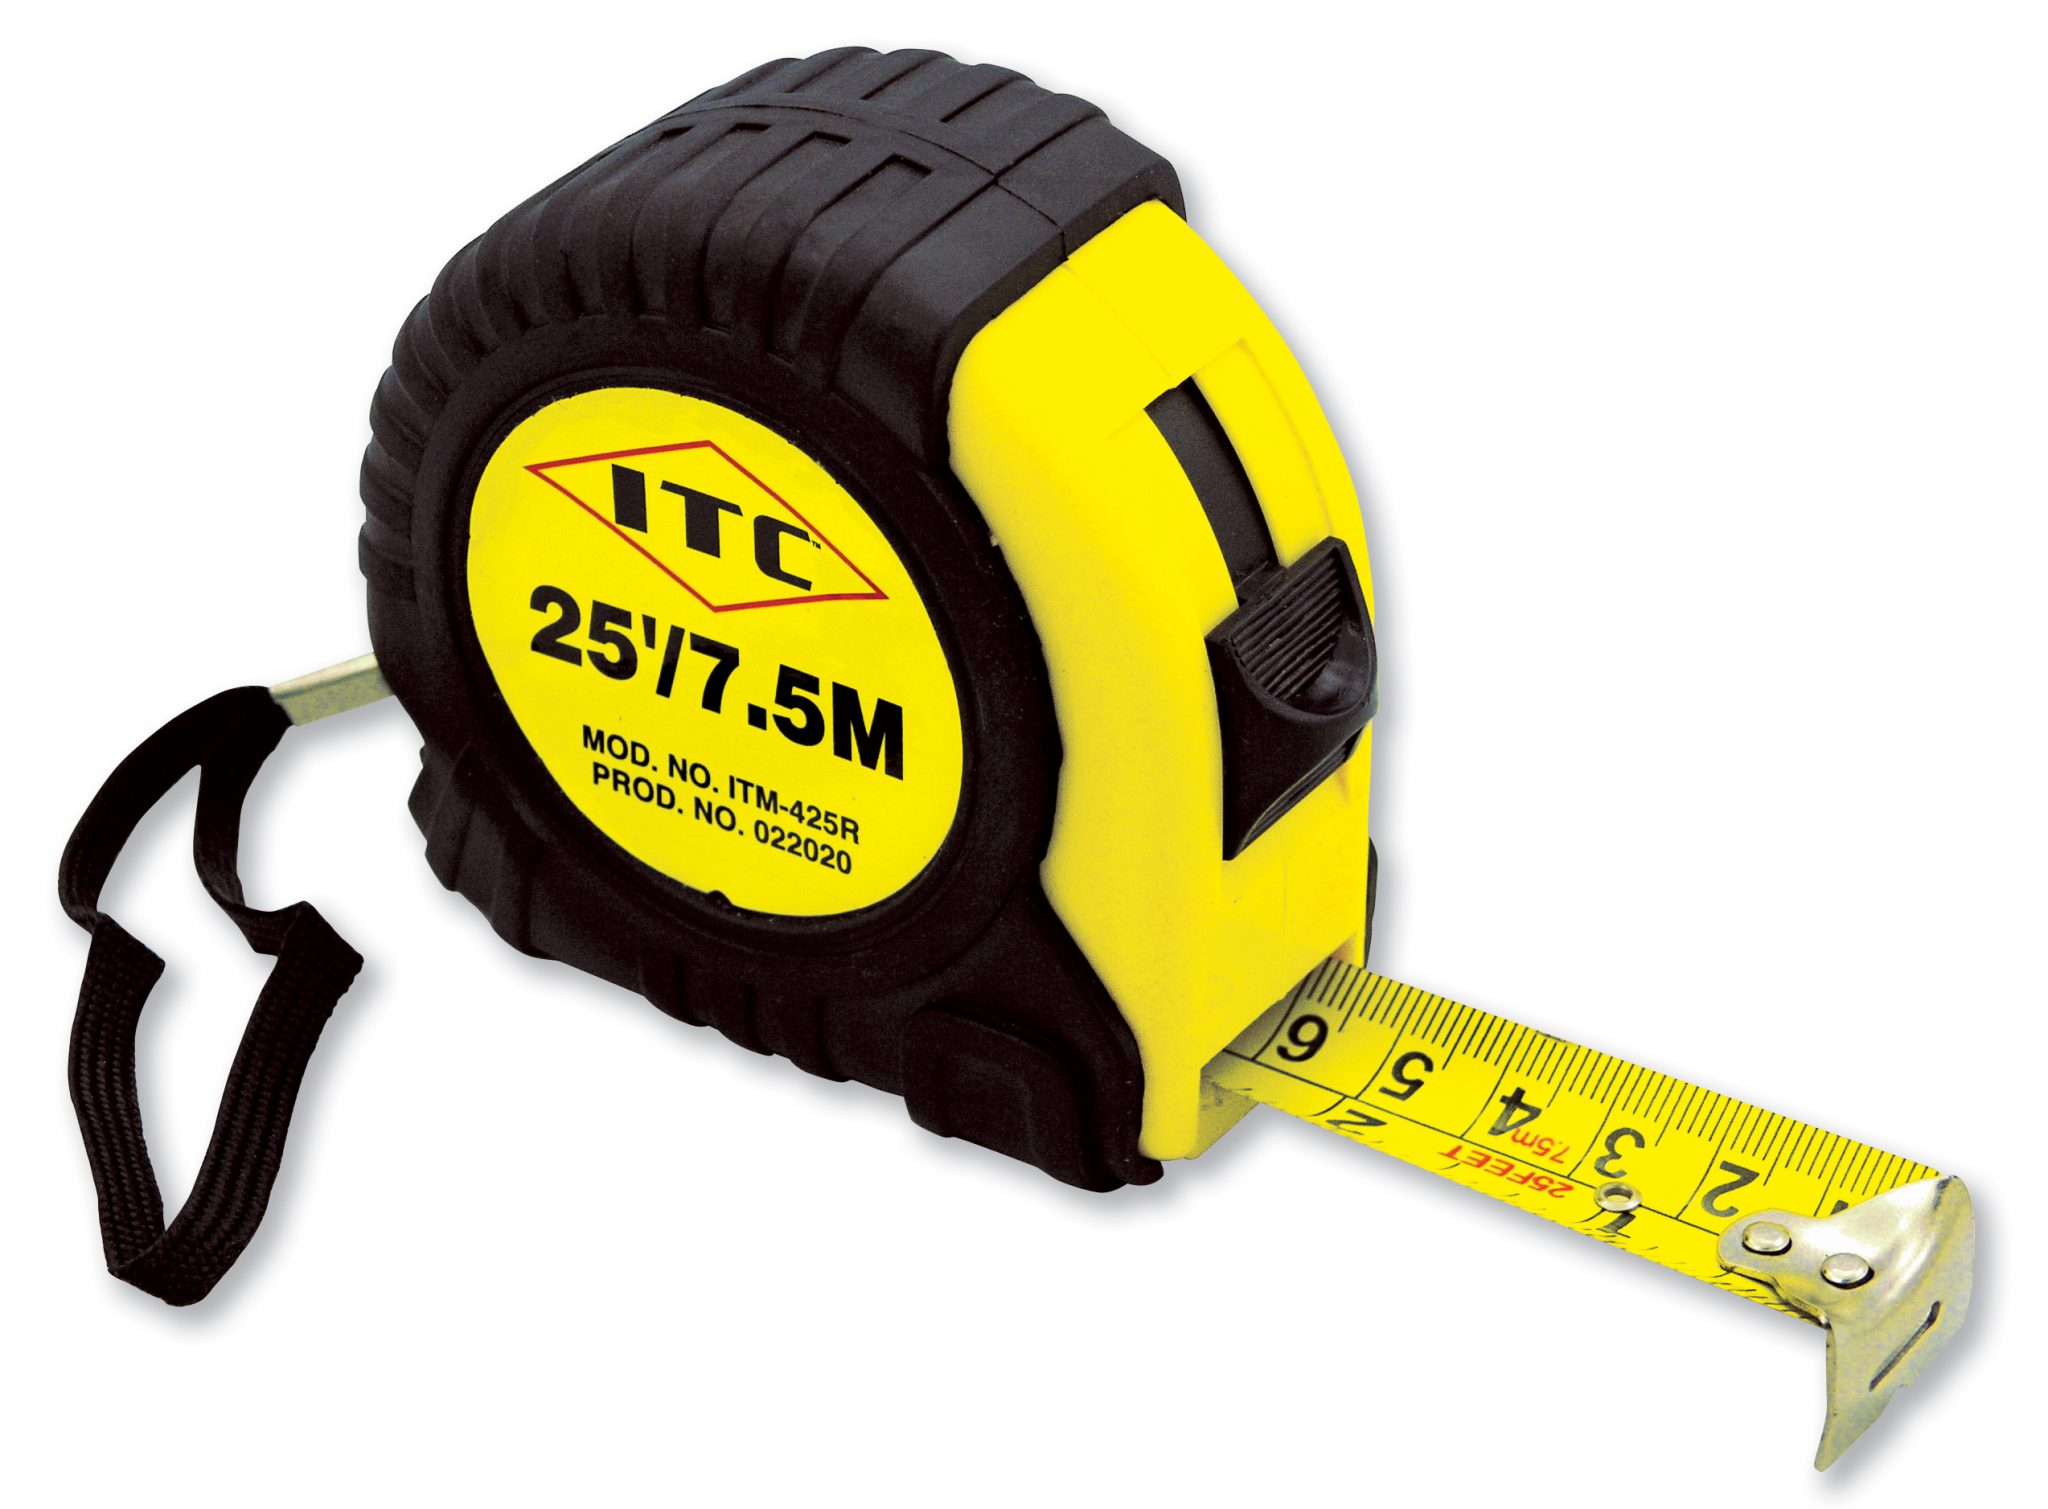
\includegraphics[scale=0.1]{tapemeasure.jpg}
            \end{figure}
        \end{frame}
        \begin{frame}
            \begin{figure}
                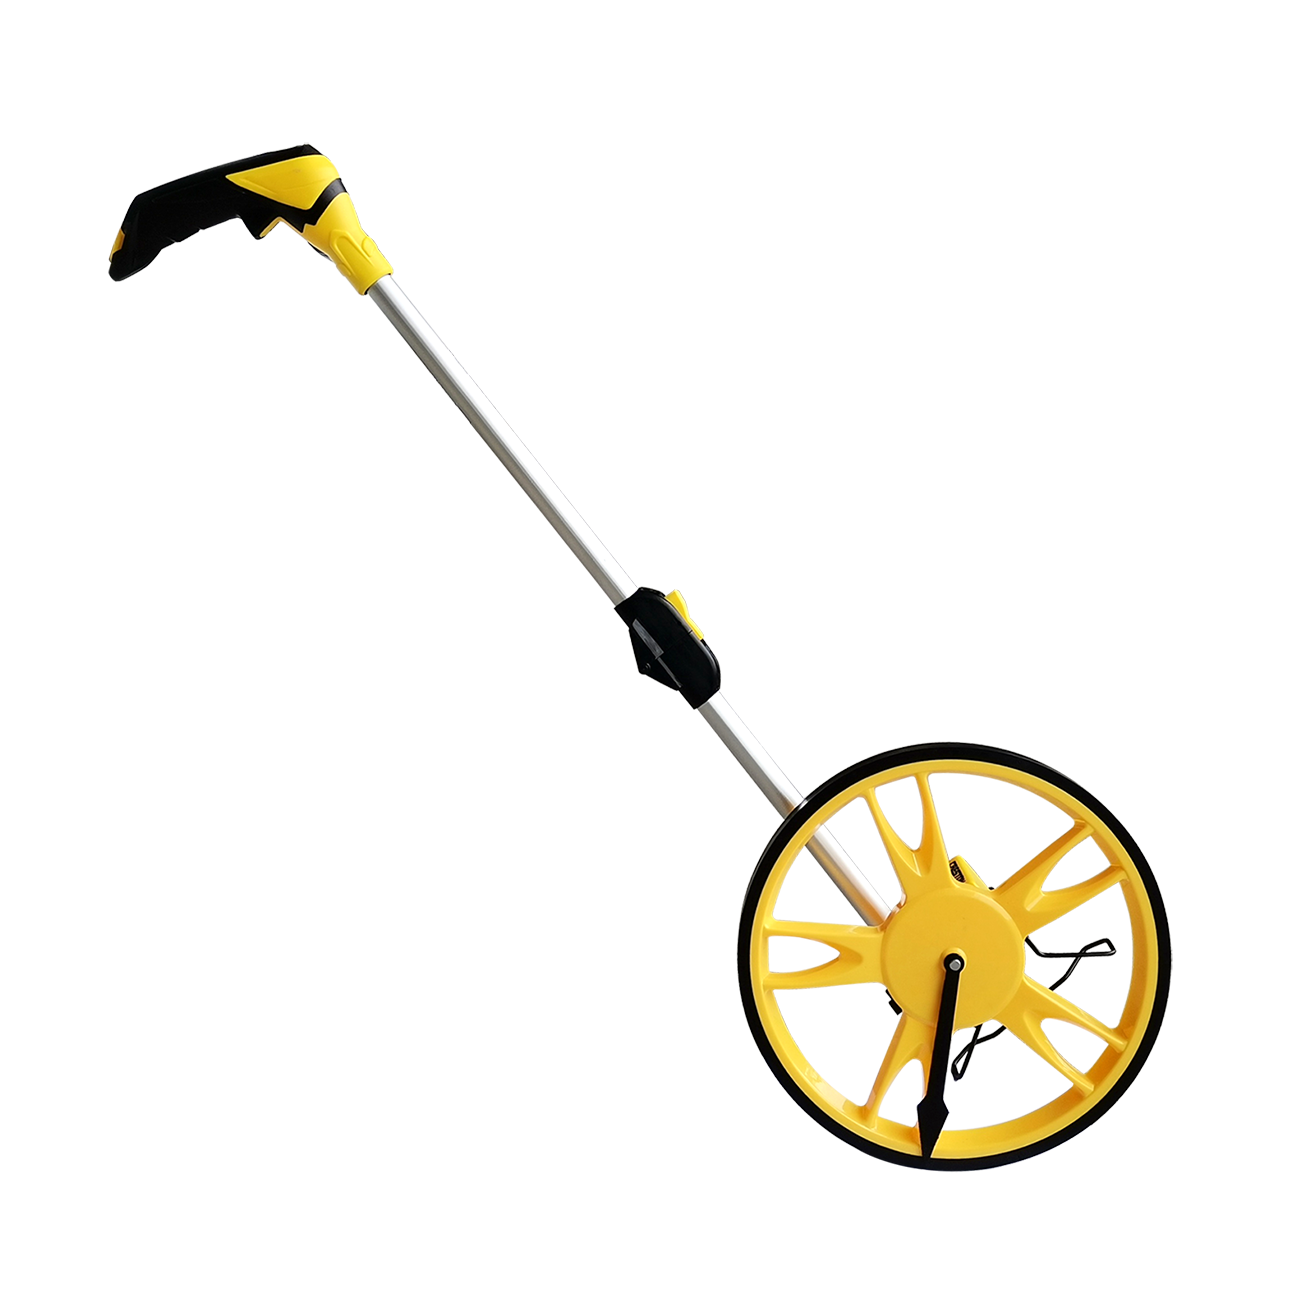
\includegraphics[scale=0.5]{rollermeasure.png}
            \end{figure}
        \end{frame}
        \begin{frame}{Units :)}{How many \textit{things} span this distance?}
            \begin{itemize}
                \item<2-> Find something to use as a unit
                \item<3-> Find out how many fit span a distance
                \begin{itemize}
                    \item Put many of these objects between and count the number
                    \item Use the same object and mark intervals of the object, count the intervals
                \end{itemize}
                \item<4-> Historically we've used things like a foot but truly make up anything
                \item<5-> If you want other people to use this unit just make sure their unit is the same as yours
            \end{itemize}
        \end{frame}
    \subsection{Measuring Devices}
        \begin{frame}{Measuring Devices}
            \begin{figure}
                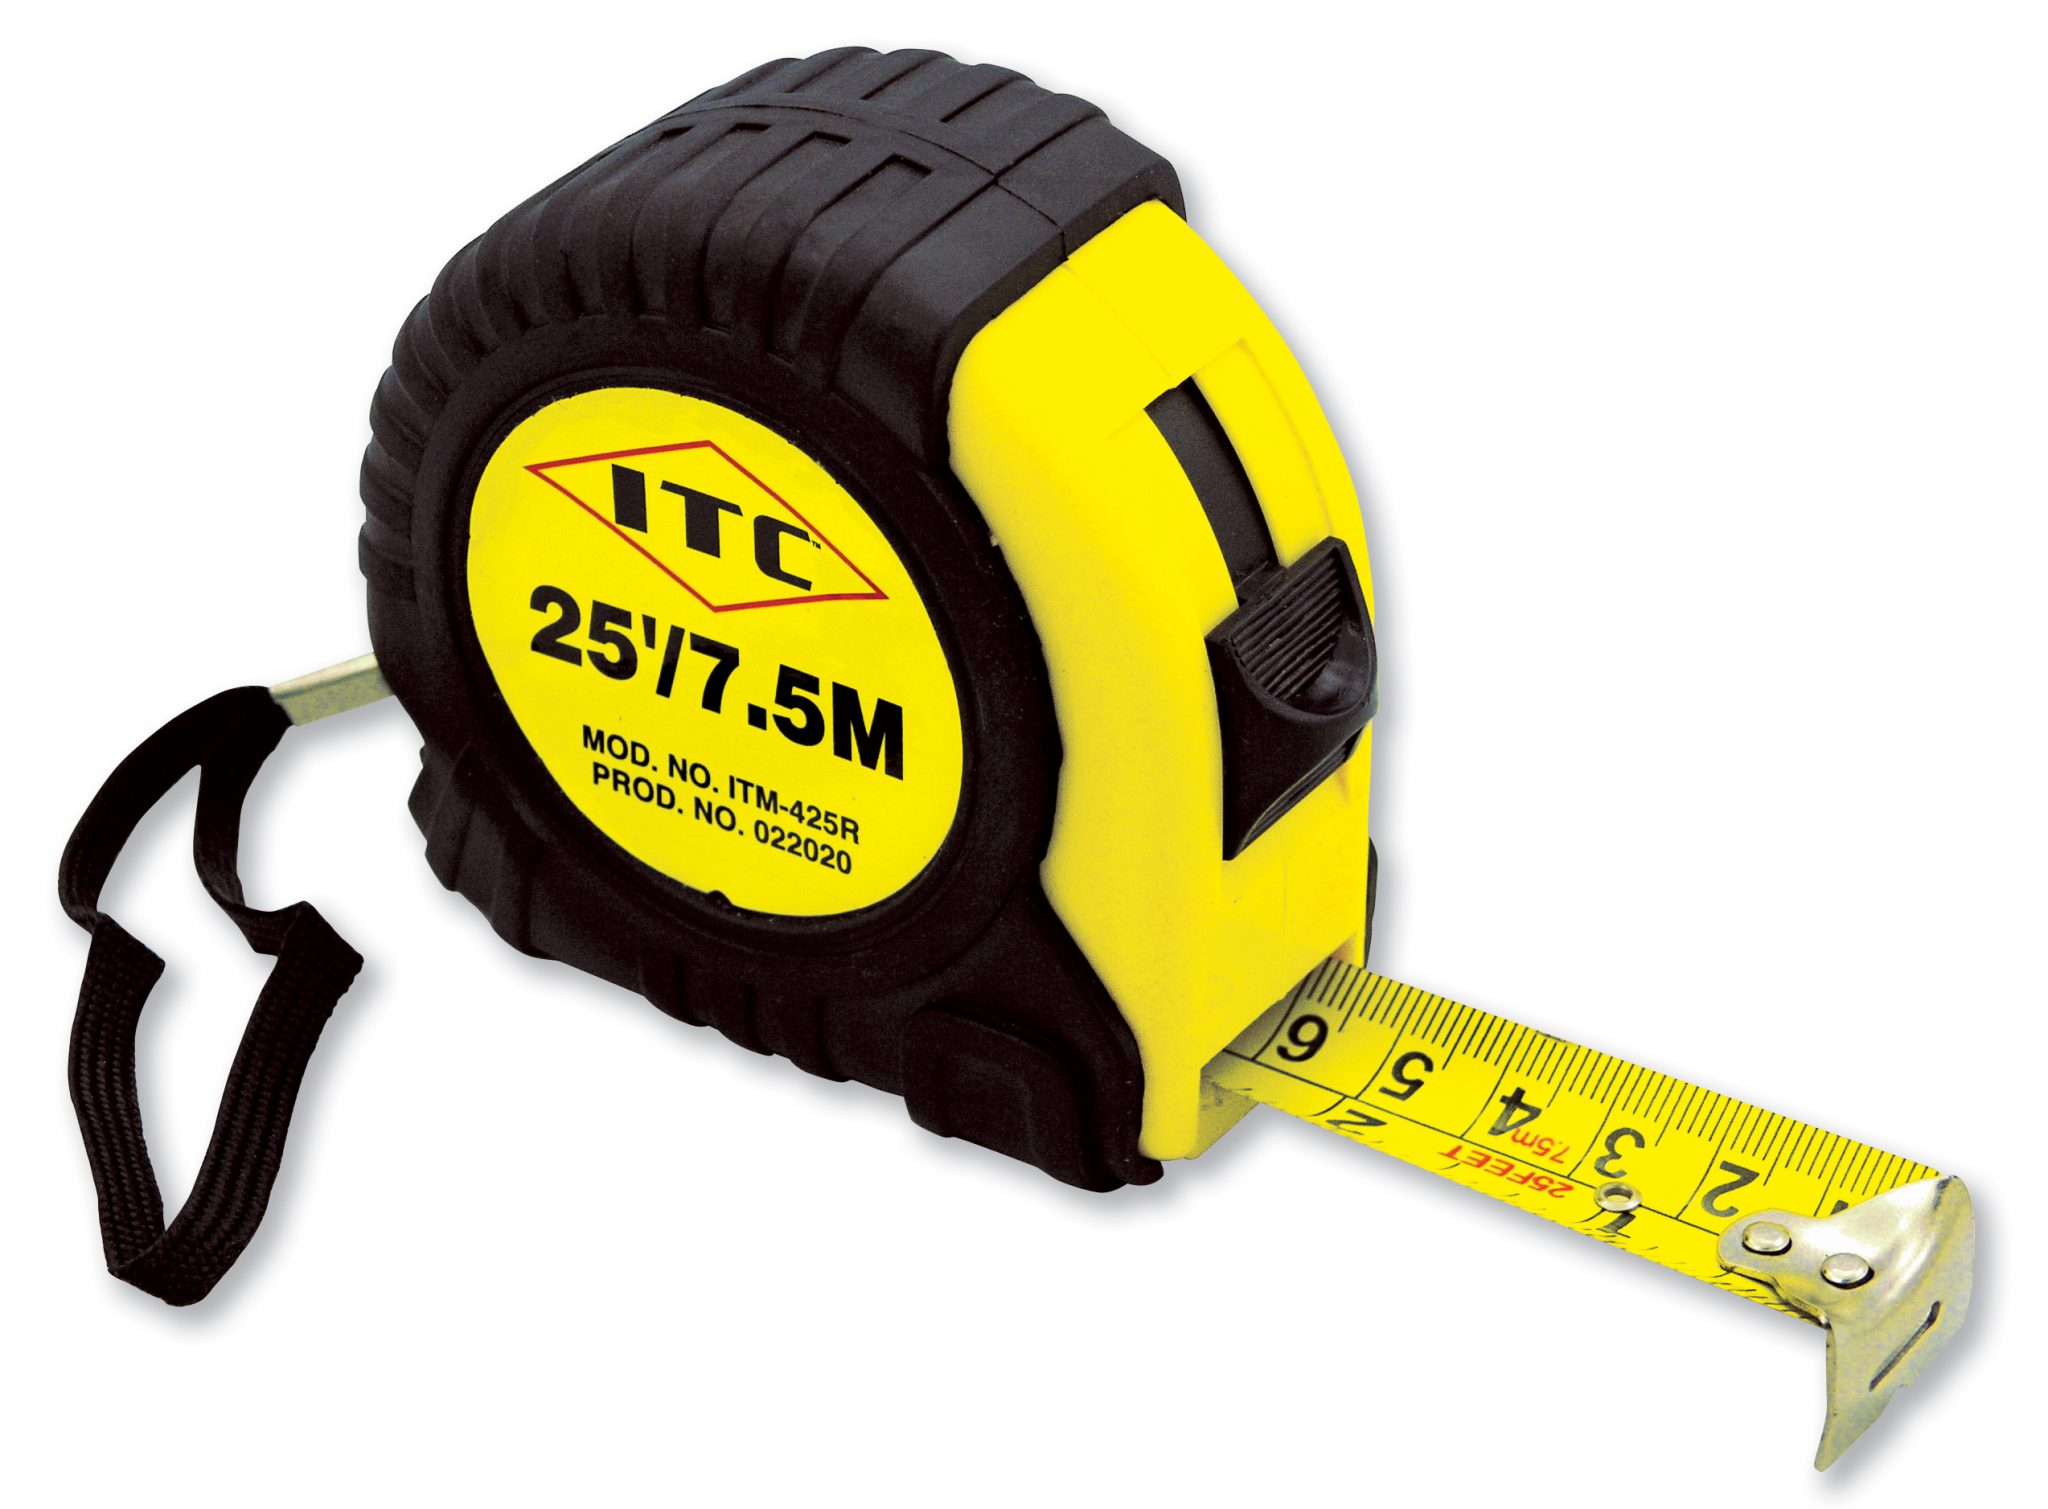
\includegraphics[scale=0.1]{tapemeasure.jpg}
                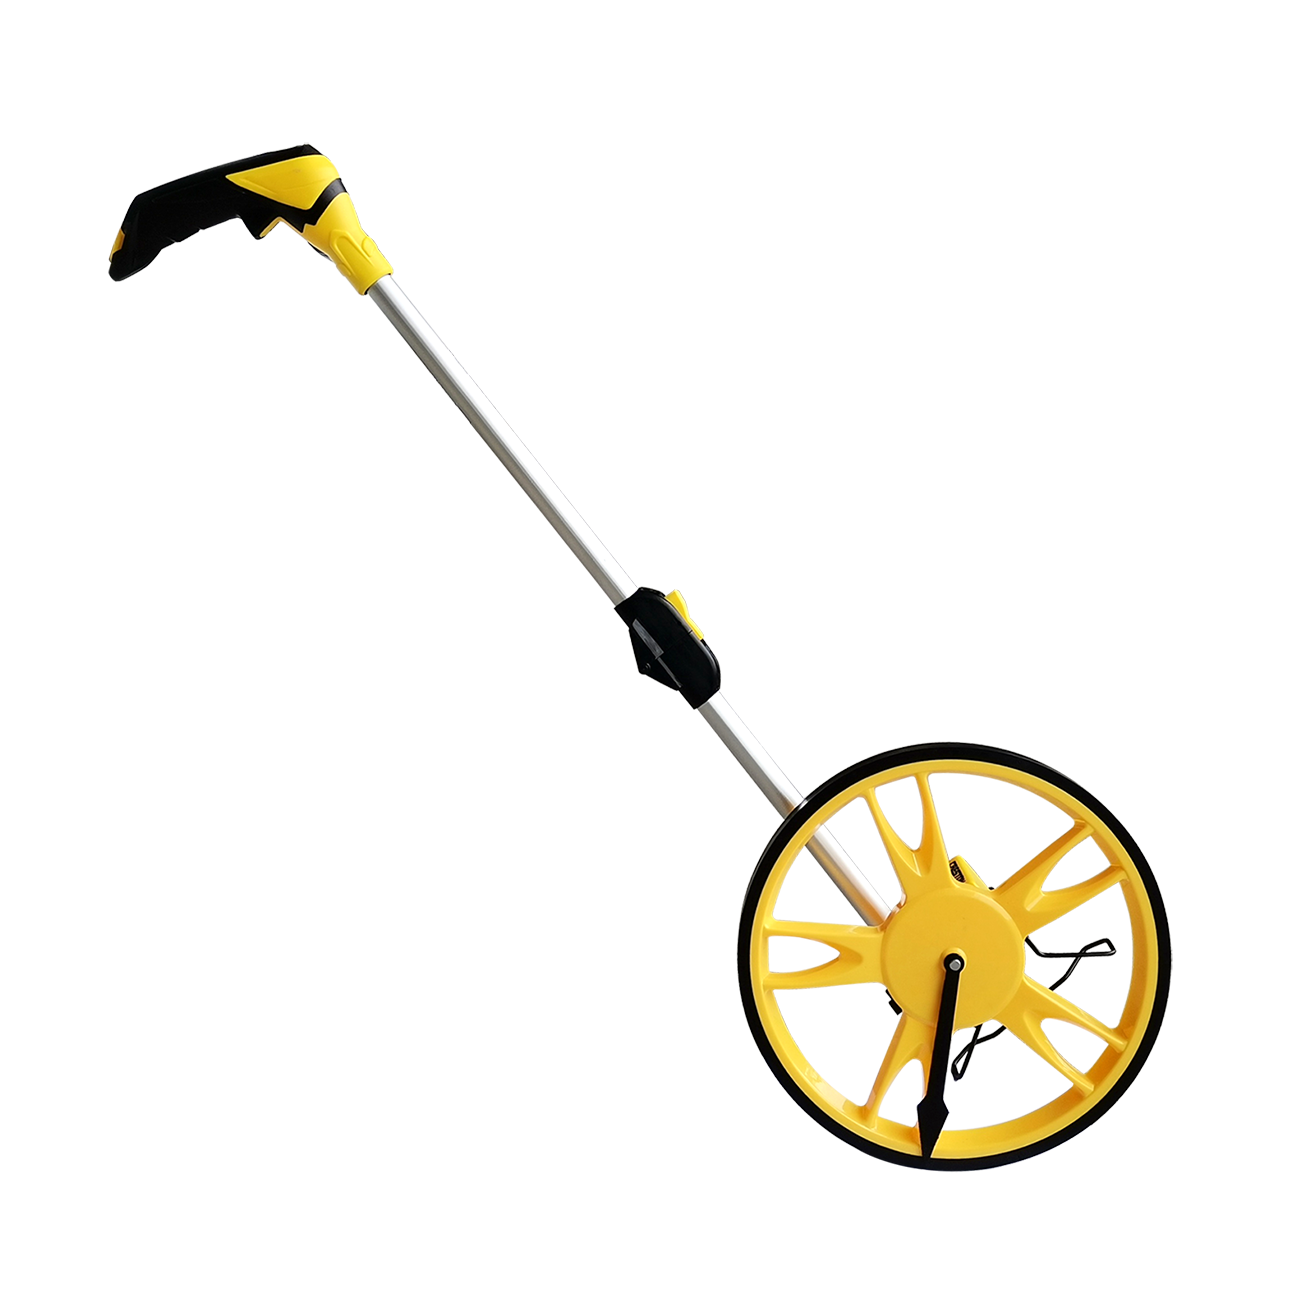
\includegraphics[scale=0.5]{rollermeasure.png}
                \caption{A tape measure and a rolly measurey thing$^1$.}
            \end{figure}
            \footnotemark{\tiny Image: https://cdn.shopify.com/s/files/1/0404/0048/6557/products/7\_CDM1001\_1024x1024\@2x.png?v=1615341175}
        \end{frame}
        \begin{frame}{how far is this fucker?}
            \begin{figure}
                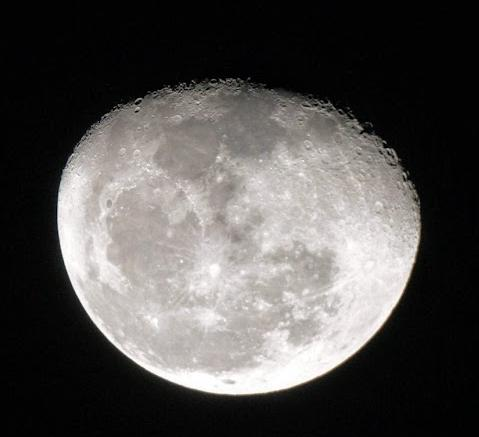
\includegraphics[scale=0.45, fbox]{moon.jpg}
                \caption{Moon$^2$.}
            \end{figure}
            \footnotemark{\tiny Image: Me :)}
        \end{frame}
\section{The Distance Ladder}
    \subsection{Background}
        \begin{frame}{The Distance Ladder}{Earth $\implies$ Moon $\implies$ Sun $\implies$ Planets $\implies$ Stars $\implies$ Galaxies} \centering
            \pause
            We need to know each distance/size in order to find out the next object's size/distance.\\
            \pause
            The goal of measuring the Earth, Moon, Sun, and stars is as old as humanity.\\ \vspace{2em}
            \small (so let's go back)
        \end{frame}
        \begin{frame}{What have we always known?} \centering
            (This is essentially the same question as what can be observed with the eyes.)
            \pause
            \begin{itemize}
                \item<2-> The Moon is closer than the Sun
            \end{itemize}
        \end{frame}
        \begin{frame} \centering
            Solar eclipses, the moon passing between the Earth and Sun
            \begin{figure}
                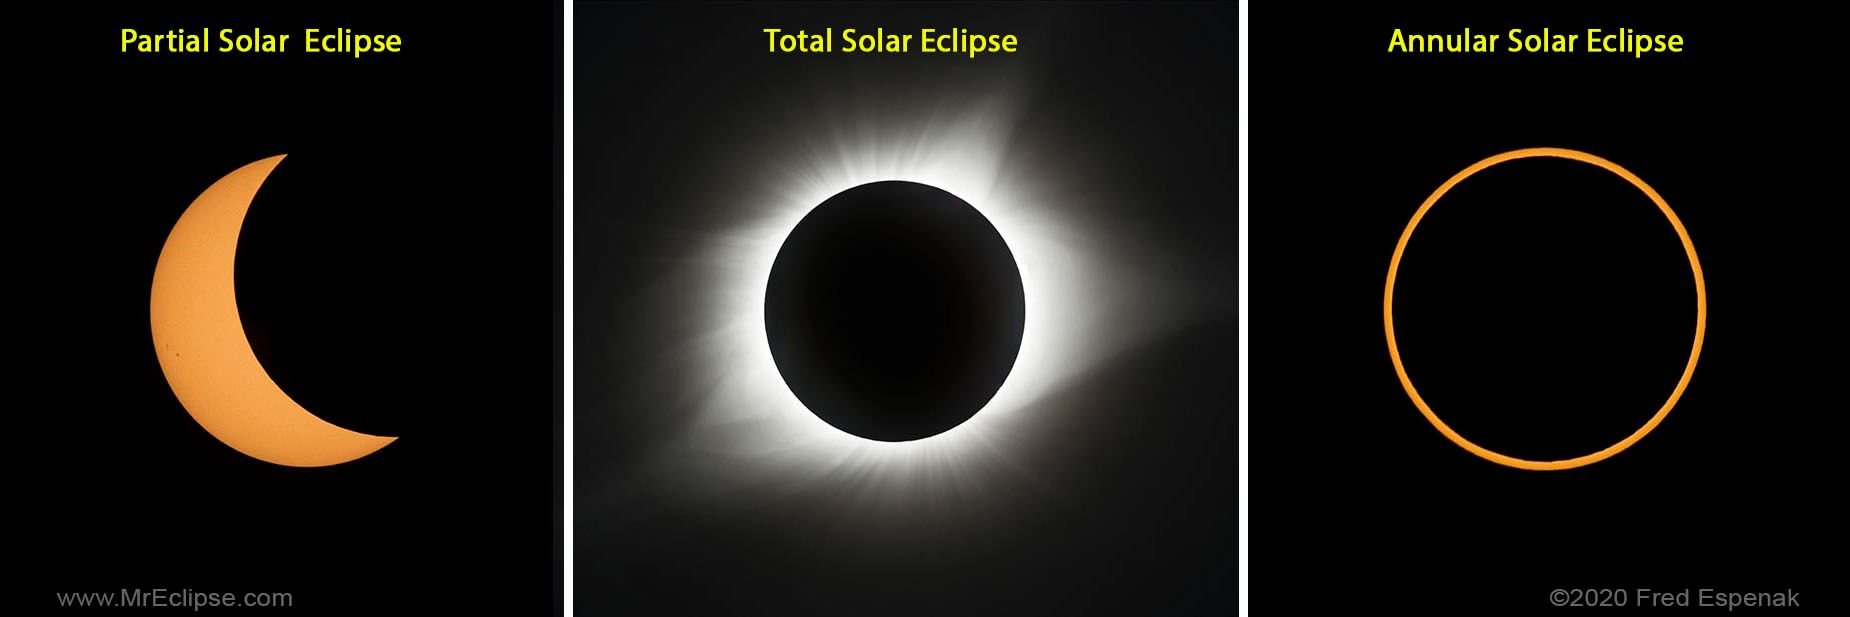
\includegraphics[scale=0.17, fbox]{eclipse.jpg}
            \caption{Partial, total, and annular eclipse images$^3$.}
            \end{figure}
            \footnotemark{\tiny Image: https://galamcdougal.blogspot.com/2022/10/solar-eclipse.html}
        \end{frame}
        \begin{frame}{What have we always known?} \centering
            (This is essentially the same question as what can be observed with the eyes.)
            \begin{itemize}
                \item The Moon is closer than the Sun (solar eclipses) and \textit{same angular size}
                \item The Earth is round
            \end{itemize}
        \end{frame}
        \begin{frame} \centering
            During a lunar eclipse, the Earth passes between a full Moon and the Sun
            \begin{figure}
                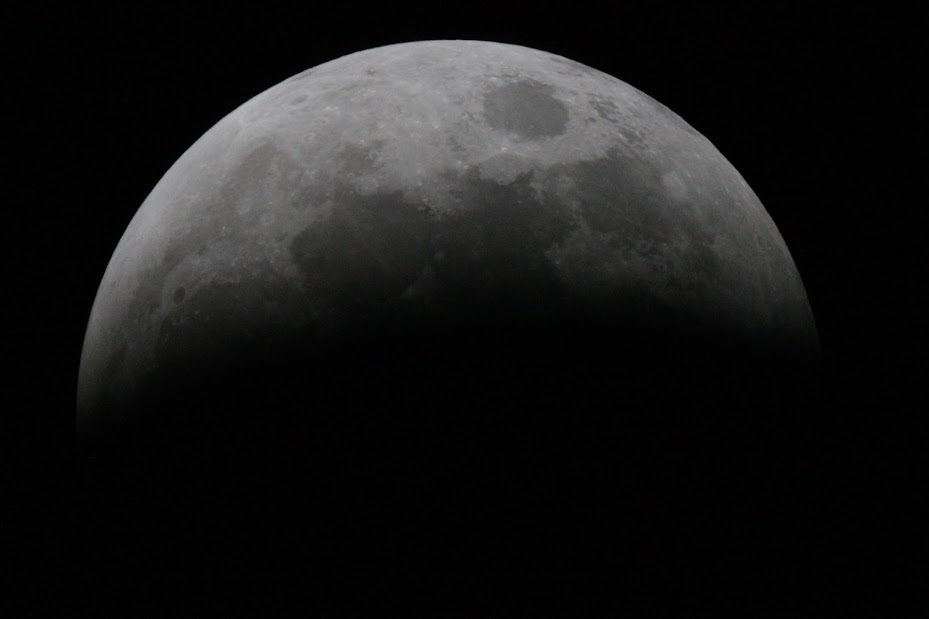
\includegraphics[scale=0.15, fbox]{lunar2.JPG}
                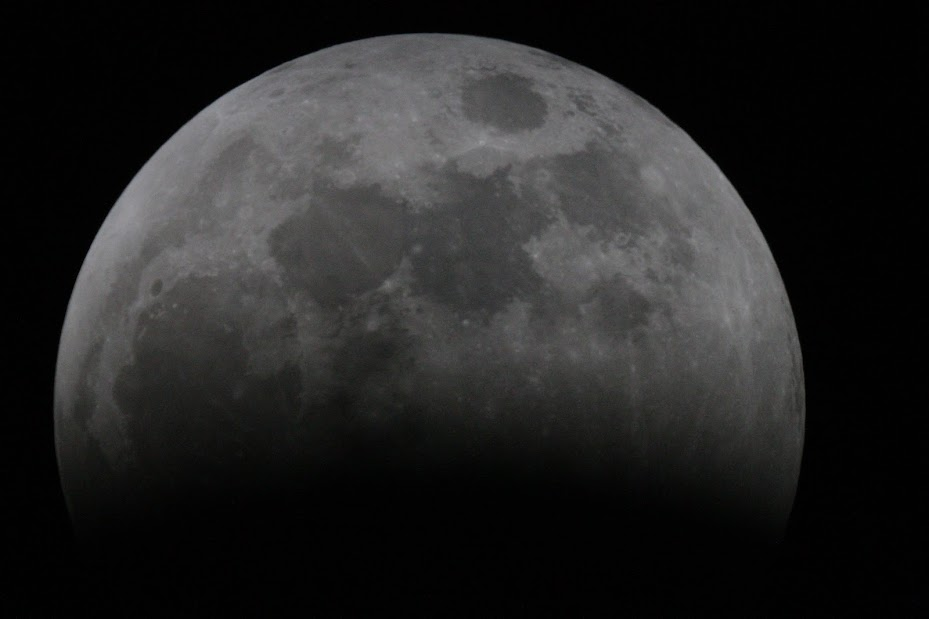
\includegraphics[scale=0.15, fbox]{lunar1.JPG}
                \caption{Two stages of a lunar eclipse$^4$.}
            \end{figure}
            \footnotemark{\tiny Images: me :)}
        \end{frame}
        \begin{frame}{What have we always known?} \centering
            (This is essentially the same question as what can be observed with the eyes.)
            \begin{itemize}
                \item The Moon is closer than the Sun (solar eclipses) and \textit{same angular size}
                \item The Earth is round (lunar eclipses)
                \item The Sun, Moon, planets, and stars are cyclical and move in `perfect circles' around the Earth on a flat plane
                \pause
                \begin{itemize}
                    \item we were wrong about this but it was a very compelling, mostly unproblematic explanation for a LONG time
                    \pause
                    \item we also knew slower moving things were farther (parallax), so we knew Jupiter and Saturn are far and Venus and Mars are close
                \end{itemize}
            \end{itemize}
        \end{frame}
        \begin{frame} \centering
            \begin{figure}
                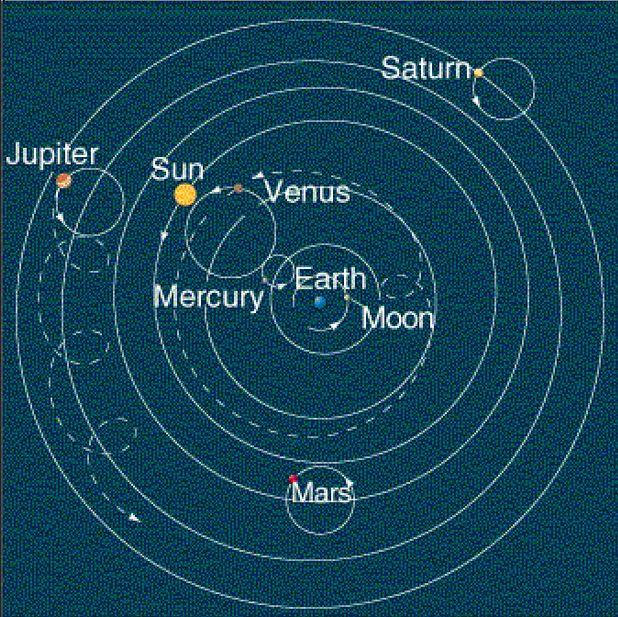
\includegraphics[scale=0.25, fbox]{geocentric.png}
                \caption{Geocentric model with subcircles that explain retrograde motion$^5$.}
            \end{figure}
            \footnotemark{\tiny Image: https://starrythoughts.weebly.com/uploads/1/6/3/0/16304784/2180964\_orig.gif}
        \end{frame}
        \begin{frame} \centering
            \begin{figure}
                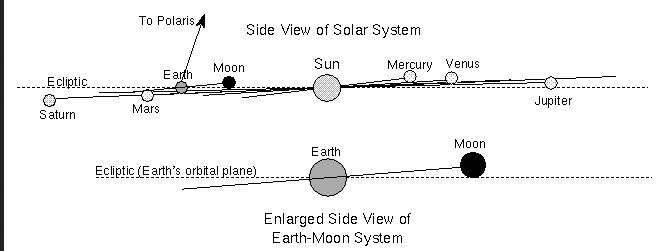
\includegraphics[scale=0.3, fbox]{ecliptic.png}\\
                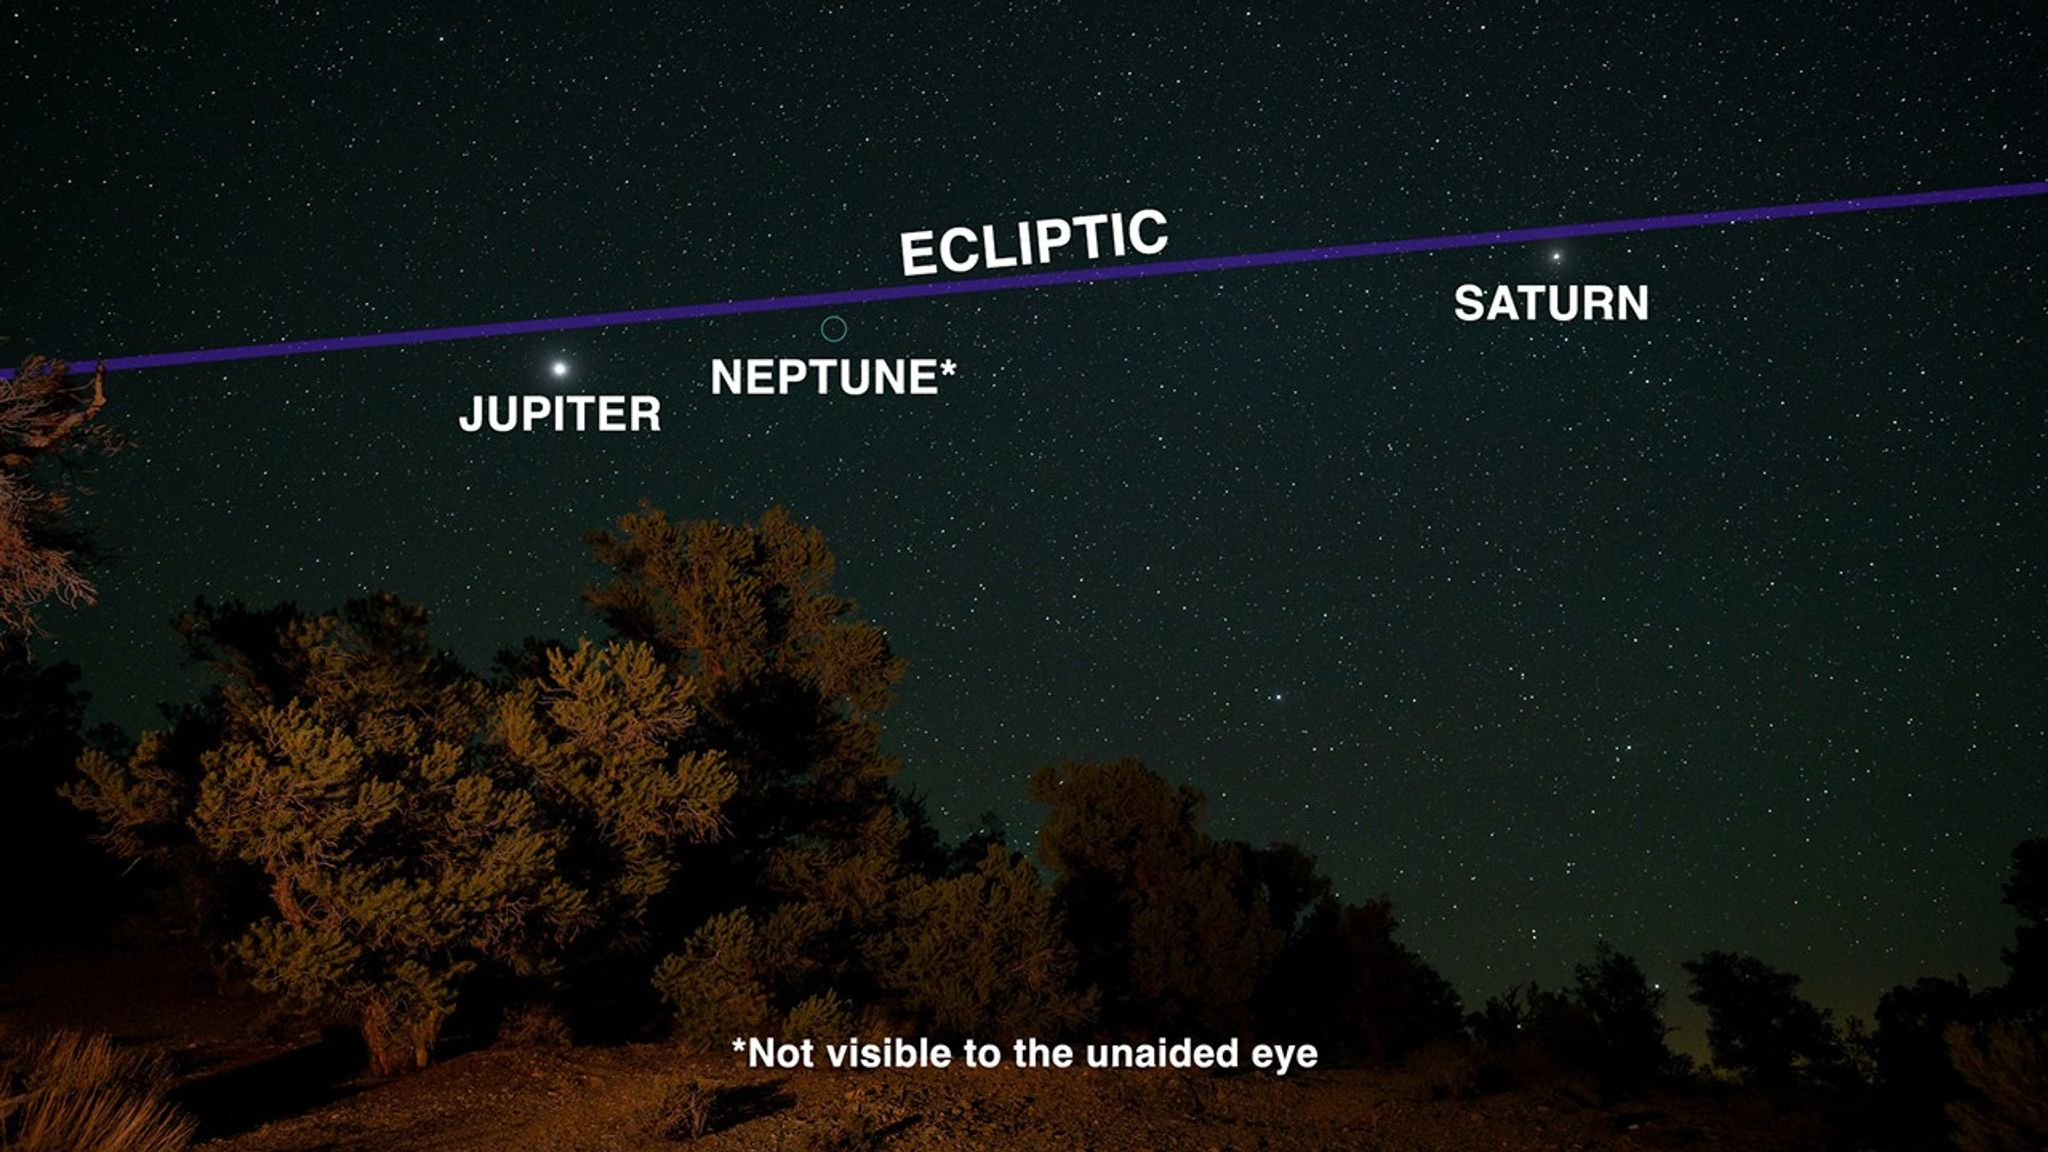
\includegraphics[scale=0.08, fbox]{eclipticsky.jpg}
                \caption{Ecliptic visuals$^6$.}
            \end{figure}
            \footnotemark{\tiny Images: https://www.astronomynotes.com/nakedeye/phases/solarsys.gif, NASA}
        \end{frame}
        \begin{frame}{In summary,}{(this information is all we needed to figure out the distance to the stars. the rest is all measurements and math)}
            \begin{itemize}
                \item The Earth is spherical
                \item The Moon is closer than the Sun and \textit{same angular size}
                \item All solar system bodies orbit in a flat plane in perfect circles around the Earth
                \pause
                \begin{itemize}
                    \item (no physics behind this, but it was a pretty viable, elegant explanation)
                \end{itemize}
            \end{itemize}
        \end{frame}
    \subsection{Earth}
        \begin{frame}{The First Recorded Attempt of Measuring Things}{Aristarchus of Samos, Greek, 270BC, Heliocentrist}
            Realized the distance of the sun would change when we observe a half-moon. Instead of starting humble with the size of the Earth bro went wacko and tried to get THIS distance first.
            \begin{figure}
                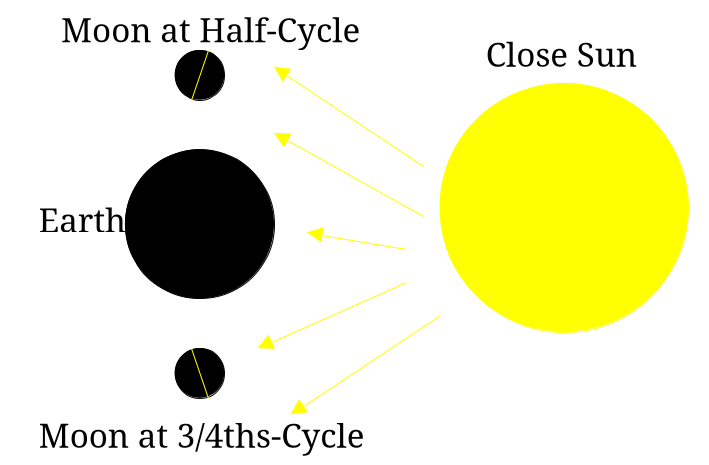
\includegraphics[scale=0.19, frame]{nearsun.png}
                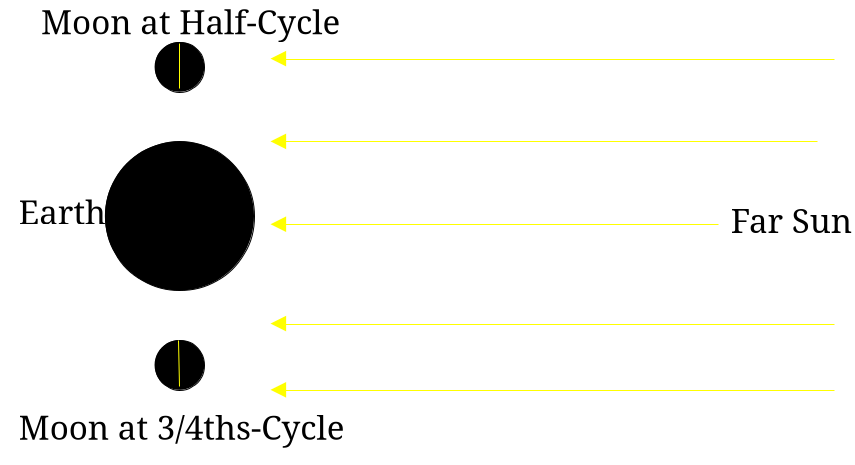
\includegraphics[scale=0.19, frame]{farsun.png}
                \caption{Near-Sun rays make a half-moon appear sooner in the lunar cycle, while far-Sun parallel rays mean half-moons happen at $\frac{1}{2}$ and $\frac{3}{4}$ in the lunar cycle.}
            \end{figure}
        \end{frame}
        \begin{frame}{Aristarchus' Method} \centering
            Measure the angle $\theta$ at exactly half-moon.
            \begin{figure}
                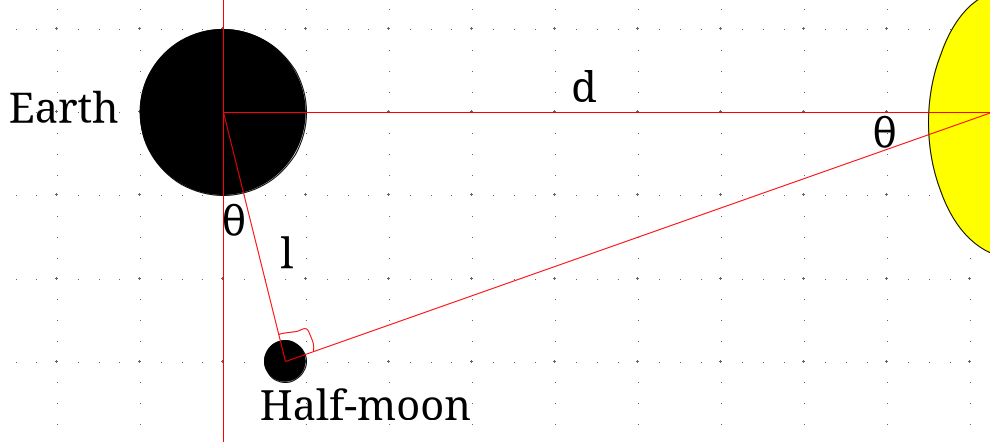
\includegraphics[scale=0.3, frame]{aristocrates.png}
            \end{figure}
            \[\sin{\theta}=\frac{l}{d} \implies \frac{l}{d}=\sin{\theta}\]
        \end{frame}
        \begin{frame}{The First Recorded Attempt of Measuring Things}{Aristarchus of Samos, Greek, 270BC, Heliocentrist}
            The issue here is incredibly precise timing --- when is it exactly half-moon?\\ \vspace{1em}
            \pause
            The lunar cycle is 29.5 days (which was known)\\
            Nowadays, we know that half-moons occur 30 mins after it reaches those 90$^\circ$ marks\\
            This meant measuring $\frac{1}{1400}$th of a lunar cycle.\\
            \vspace{1em}
            \pause
            Aristarchus measured $87^\circ$, meaning $\frac{l}{d}=\sin{(90^\circ-87^\circ)}=19.1$ the Sun is 19x farther away than the Moon.\\
            In reality, this half-moon angle is 89.88$^\circ$, which gives a much larger number: the Sun is 409x farther away than the Moon.
        \end{frame}
        \begin{frame}{The First Recorded Attempt of Measuring Things}{Aristarchus of Samos, Greek, 270BC, Heliocentrist} \centering
            good effort dipshit
        \end{frame}
        \begin{frame}{Eratosthenes and the Size of the Earth}{Greece, 230BC} \centering
            The first good measurement of the size of the Earth
            \pause
            \begin{figure}
                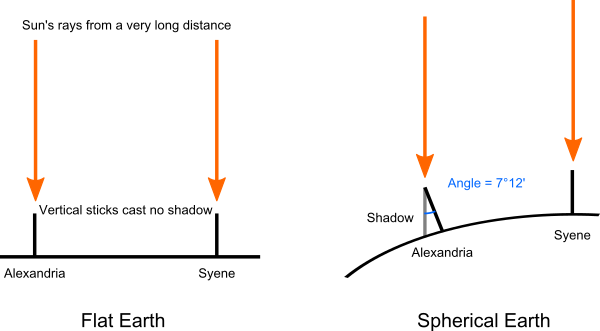
\includegraphics[scale=0.35, frame]{eritosthenesdiagram.png}
                \caption{Eratosthenes' experimental setup$^7$.}
            \end{figure}
            \footnotemark{\tiny Image: https://www.mezzacotta.net/100proofs/images/002-SyeneAlexandria.png}
        \end{frame}
        \begin{frame}{Eratosthenes and the Size of the Earth}{Greece, 230BC} \centering
            Eratosthenes knew the city of Syene was on the Tropic of Cancer (no shadows on summer solstice, sun right overhead)\\ \vspace{1em}
            
            He also knew the distance between Alexandria and Syene\\

            \begin{figure}
                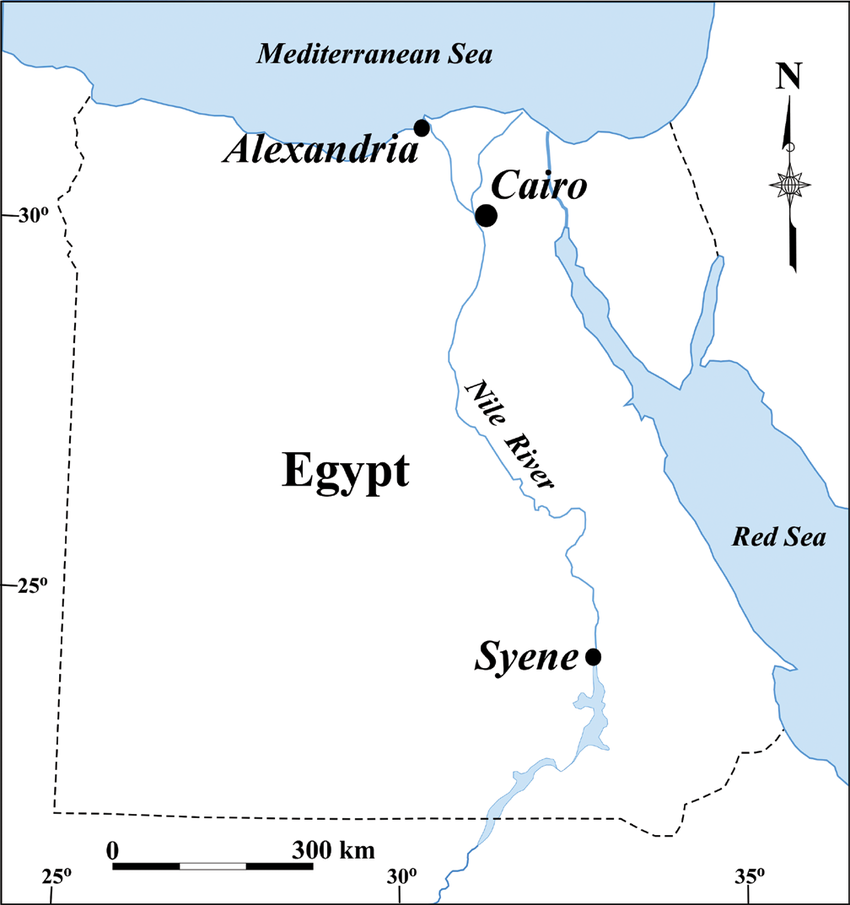
\includegraphics[scale=0.1, frame]{egyptmap.png}
                \caption{Alexandria and Syene along the Nile River in Egypt$^8$.}
            \end{figure}
            \footnotemark{\tiny Image: https://www.researchgate.net/profile/Alok-Kumar-111/publication/253596660/figure/fig2/}
        \end{frame}
        \begin{frame}{Eratosthenes' Method}
            \begin{columns}
                \begin{column}{0.5\linewidth}
                    \begin{figure}
                        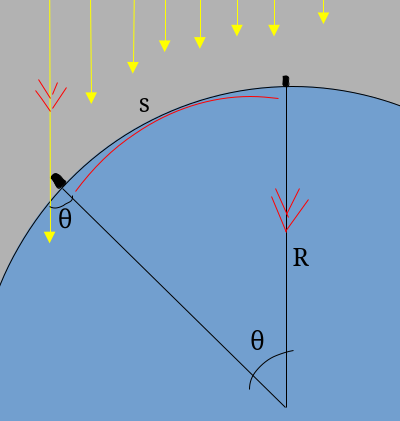
\includegraphics[scale=0.4, frame]{earthdiam.png}
                    \end{figure}
                \end{column}
                \begin{column}{0.5\linewidth}
                    Arc length:\\
                    \[s=\frac{{\pi}R\theta}{180^\circ}\]
                    Rearrange for R, Earth's radius:\\
                    \[R=\frac{180s}{\pi\theta}\]
                    $s$ was already known from geographical data, and $\theta$ was measureable from shadows cast in Alexandria.
                \end{column}
            \end{columns}
        \end{frame}
        \begin{frame}{Eratosthenes and the Size of the Earth}{Greece, 230BC} \centering
            To avoid doing difficult division with $\pi$, he opted to calculate the circumference, not the radius:
            \[C=2{\pi}R=\frac{360s}{\theta}\]
            To which he found a value of 252,000 stadia.\\
            In ancient Greece, they used a unit called a `stade'. We don't really know how big a stade was, but we estimate 1 stade is about 525ft, making his calculation \textit{less than 1\% off.}\\ \vspace{1em}
            Eratosthenes: 25,050mi.\\
            Modern value: 24,901mi.
        \end{frame}
    \subsection{Moon}
        \begin{frame}{Hipparchus and the Distance to the Moon}{Greece, 189BC} \centering
            Looking at a solar eclipse from two different places allowed for the calculation of the distance to the moon
        \end{frame}
    \subsection{Sun}
        \begin{frame}{How far is the sun?}{This would've been really complicated math, but the moon and the sun happen to be the same apparent size} \centering
            Because the moon and the sun are the same apparent size in the sky, and since we know how big and far the moon is\ldots\\
            We know that if the sun is $x$ times further than the moon, that is must also be $x$ times larger.\\
            % Add more here, I might not know what I'm talking about. I need to read more on this
        \end{frame}
    \subsection{Planets}
    \subsection{Stars}
        \begin{frame}{How far are the stars?}{We can only calculate this if we know the astronomical unit (AU)}
            % This needs diagrams or something, this is the most cool, classic example of parallax measurements
        \end{frame}
    \subsection{Galaxies}
        \begin{frame}{How far are galaxies?} \centering
            Galaxies are so distant that they have no apparent motion due to parallax. It's too small to measure.\\

            This is where all the really neat fun geometry breaks down and it just gets to grueling modern science of measuring light and doing really hard math.

            % How do we know how far galaxies are from us? That's a great question. I don't know, other than redshift and spectroscopy.
        \end{frame}

\end{document}
